\PassOptionsToPackage{unicode=true}{hyperref} % options for packages loaded elsewhere
\PassOptionsToPackage{hyphens}{url}
%
\documentclass[ignorenonframetext,]{beamer}
\usepackage{pgfpages}
\setbeamertemplate{caption}[numbered]
\setbeamertemplate{caption label separator}{: }
\setbeamercolor{caption name}{fg=normal text.fg}
\beamertemplatenavigationsymbolsempty
\usepackage{lmodern}
\usepackage{amssymb,amsmath}
\usepackage{ifxetex,ifluatex}
\usepackage{fixltx2e} % provides \textsubscript
\ifnum 0\ifxetex 1\fi\ifluatex 1\fi=0 % if pdftex
  \usepackage[T1]{fontenc}
  \usepackage[utf8]{inputenc}
  \usepackage{textcomp} % provides euro and other symbols
\else % if luatex or xelatex
  \usepackage{unicode-math}
  \defaultfontfeatures{Ligatures=TeX,Scale=MatchLowercase}
\fi
\usetheme[]{CambridgeUS}
\usecolortheme{beaver}
\usefonttheme{structurebold}
% use upquote if available, for straight quotes in verbatim environments
\IfFileExists{upquote.sty}{\usepackage{upquote}}{}
% use microtype if available
\IfFileExists{microtype.sty}{%
\usepackage[]{microtype}
\UseMicrotypeSet[protrusion]{basicmath} % disable protrusion for tt fonts
}{}
\IfFileExists{parskip.sty}{%
\usepackage{parskip}
}{% else
\setlength{\parindent}{0pt}
\setlength{\parskip}{6pt plus 2pt minus 1pt}
}
\usepackage{hyperref}
\hypersetup{
            pdftitle={B1 - Das Arbeiten mit OSM Daten},
            pdfauthor={Jan-Philipp Kolb},
            pdfborder={0 0 0},
            breaklinks=true}
\urlstyle{same}  % don't use monospace font for urls
\newif\ifbibliography
\usepackage{color}
\usepackage{fancyvrb}
\newcommand{\VerbBar}{|}
\newcommand{\VERB}{\Verb[commandchars=\\\{\}]}
\DefineVerbatimEnvironment{Highlighting}{Verbatim}{commandchars=\\\{\}}
% Add ',fontsize=\small' for more characters per line
\usepackage{framed}
\definecolor{shadecolor}{RGB}{248,248,248}
\newenvironment{Shaded}{\begin{snugshade}}{\end{snugshade}}
\newcommand{\AlertTok}[1]{\textcolor[rgb]{0.94,0.16,0.16}{#1}}
\newcommand{\AnnotationTok}[1]{\textcolor[rgb]{0.56,0.35,0.01}{\textbf{\textit{#1}}}}
\newcommand{\AttributeTok}[1]{\textcolor[rgb]{0.77,0.63,0.00}{#1}}
\newcommand{\BaseNTok}[1]{\textcolor[rgb]{0.00,0.00,0.81}{#1}}
\newcommand{\BuiltInTok}[1]{#1}
\newcommand{\CharTok}[1]{\textcolor[rgb]{0.31,0.60,0.02}{#1}}
\newcommand{\CommentTok}[1]{\textcolor[rgb]{0.56,0.35,0.01}{\textit{#1}}}
\newcommand{\CommentVarTok}[1]{\textcolor[rgb]{0.56,0.35,0.01}{\textbf{\textit{#1}}}}
\newcommand{\ConstantTok}[1]{\textcolor[rgb]{0.00,0.00,0.00}{#1}}
\newcommand{\ControlFlowTok}[1]{\textcolor[rgb]{0.13,0.29,0.53}{\textbf{#1}}}
\newcommand{\DataTypeTok}[1]{\textcolor[rgb]{0.13,0.29,0.53}{#1}}
\newcommand{\DecValTok}[1]{\textcolor[rgb]{0.00,0.00,0.81}{#1}}
\newcommand{\DocumentationTok}[1]{\textcolor[rgb]{0.56,0.35,0.01}{\textbf{\textit{#1}}}}
\newcommand{\ErrorTok}[1]{\textcolor[rgb]{0.64,0.00,0.00}{\textbf{#1}}}
\newcommand{\ExtensionTok}[1]{#1}
\newcommand{\FloatTok}[1]{\textcolor[rgb]{0.00,0.00,0.81}{#1}}
\newcommand{\FunctionTok}[1]{\textcolor[rgb]{0.00,0.00,0.00}{#1}}
\newcommand{\ImportTok}[1]{#1}
\newcommand{\InformationTok}[1]{\textcolor[rgb]{0.56,0.35,0.01}{\textbf{\textit{#1}}}}
\newcommand{\KeywordTok}[1]{\textcolor[rgb]{0.13,0.29,0.53}{\textbf{#1}}}
\newcommand{\NormalTok}[1]{#1}
\newcommand{\OperatorTok}[1]{\textcolor[rgb]{0.81,0.36,0.00}{\textbf{#1}}}
\newcommand{\OtherTok}[1]{\textcolor[rgb]{0.56,0.35,0.01}{#1}}
\newcommand{\PreprocessorTok}[1]{\textcolor[rgb]{0.56,0.35,0.01}{\textit{#1}}}
\newcommand{\RegionMarkerTok}[1]{#1}
\newcommand{\SpecialCharTok}[1]{\textcolor[rgb]{0.00,0.00,0.00}{#1}}
\newcommand{\SpecialStringTok}[1]{\textcolor[rgb]{0.31,0.60,0.02}{#1}}
\newcommand{\StringTok}[1]{\textcolor[rgb]{0.31,0.60,0.02}{#1}}
\newcommand{\VariableTok}[1]{\textcolor[rgb]{0.00,0.00,0.00}{#1}}
\newcommand{\VerbatimStringTok}[1]{\textcolor[rgb]{0.31,0.60,0.02}{#1}}
\newcommand{\WarningTok}[1]{\textcolor[rgb]{0.56,0.35,0.01}{\textbf{\textit{#1}}}}
\usepackage{graphicx,grffile}
\makeatletter
\def\maxwidth{\ifdim\Gin@nat@width>\linewidth\linewidth\else\Gin@nat@width\fi}
\def\maxheight{\ifdim\Gin@nat@height>\textheight\textheight\else\Gin@nat@height\fi}
\makeatother
% Scale images if necessary, so that they will not overflow the page
% margins by default, and it is still possible to overwrite the defaults
% using explicit options in \includegraphics[width, height, ...]{}
\setkeys{Gin}{width=\maxwidth,height=\maxheight,keepaspectratio}
% Prevent slide breaks in the middle of a paragraph:
\widowpenalties 1 10000
\raggedbottom
\setbeamertemplate{part page}{
\centering
\begin{beamercolorbox}[sep=16pt,center]{part title}
  \usebeamerfont{part title}\insertpart\par
\end{beamercolorbox}
}
\setbeamertemplate{section page}{
\centering
\begin{beamercolorbox}[sep=12pt,center]{part title}
  \usebeamerfont{section title}\insertsection\par
\end{beamercolorbox}
}
\setbeamertemplate{subsection page}{
\centering
\begin{beamercolorbox}[sep=8pt,center]{part title}
  \usebeamerfont{subsection title}\insertsubsection\par
\end{beamercolorbox}
}
\AtBeginPart{
  \frame{\partpage}
}
\AtBeginSection{
  \ifbibliography
  \else
    \frame{\sectionpage}
  \fi
}
\AtBeginSubsection{
  \frame{\subsectionpage}
}
\setlength{\emergencystretch}{3em}  % prevent overfull lines
\providecommand{\tightlist}{%
  \setlength{\itemsep}{0pt}\setlength{\parskip}{0pt}}
\setcounter{secnumdepth}{0}

% set default figure placement to htbp
\makeatletter
\def\fps@figure{htbp}
\makeatother


\title{B1 - Das Arbeiten mit OSM Daten}
\author{Jan-Philipp Kolb}
\date{22 Oktober 2018}

\begin{document}
\frame{\titlepage}

\begin{frame}{Inhalt dieses Abschnitts}
\protect\hypertarget{inhalt-dieses-abschnitts}{}

\begin{itemize}
\tightlist
\item
  Vorstellung des Openstreetmap (OSM) Projekts
\item
  Welche OSM-Daten sind erhältlich?
\item
  Vorstellung von Forschung die mit OSM-Daten durchgeführt wurde
\end{itemize}

\end{frame}

\begin{frame}{\href{http://www.openstreetmap.de/}{OpenStreetMap}
Projekt}
\protect\hypertarget{openstreetmap-projekt}{}

\begin{block}{\url{http://www.openstreetmap.de/}}

\begin{quote}
OpenStreetMap.org ist ein im Jahre 2004 gegründetes internationales
Projekt mit dem Ziel, eine freie Weltkarte zu erschaffen. Dafür sammeln
wir weltweit Daten über Straßen, Eisenbahnen, Flüsse, Wälder, Häuser und
vieles mehr.
\end{quote}

\end{block}

\end{frame}

\begin{frame}{OpenStreetMap}
\protect\hypertarget{openstreetmap}{}

\begin{block}{\href{https://en.wikipedia.org/wiki/OpenStreetMap}{\textbf{Wikipedia
- OpenStreetMap}}}

\begin{quote}
OpenStreetMap (OSM) ist ein kollaboratives Projekt um eine editierbare
Weltkarte zu erzeugen.
\end{quote}

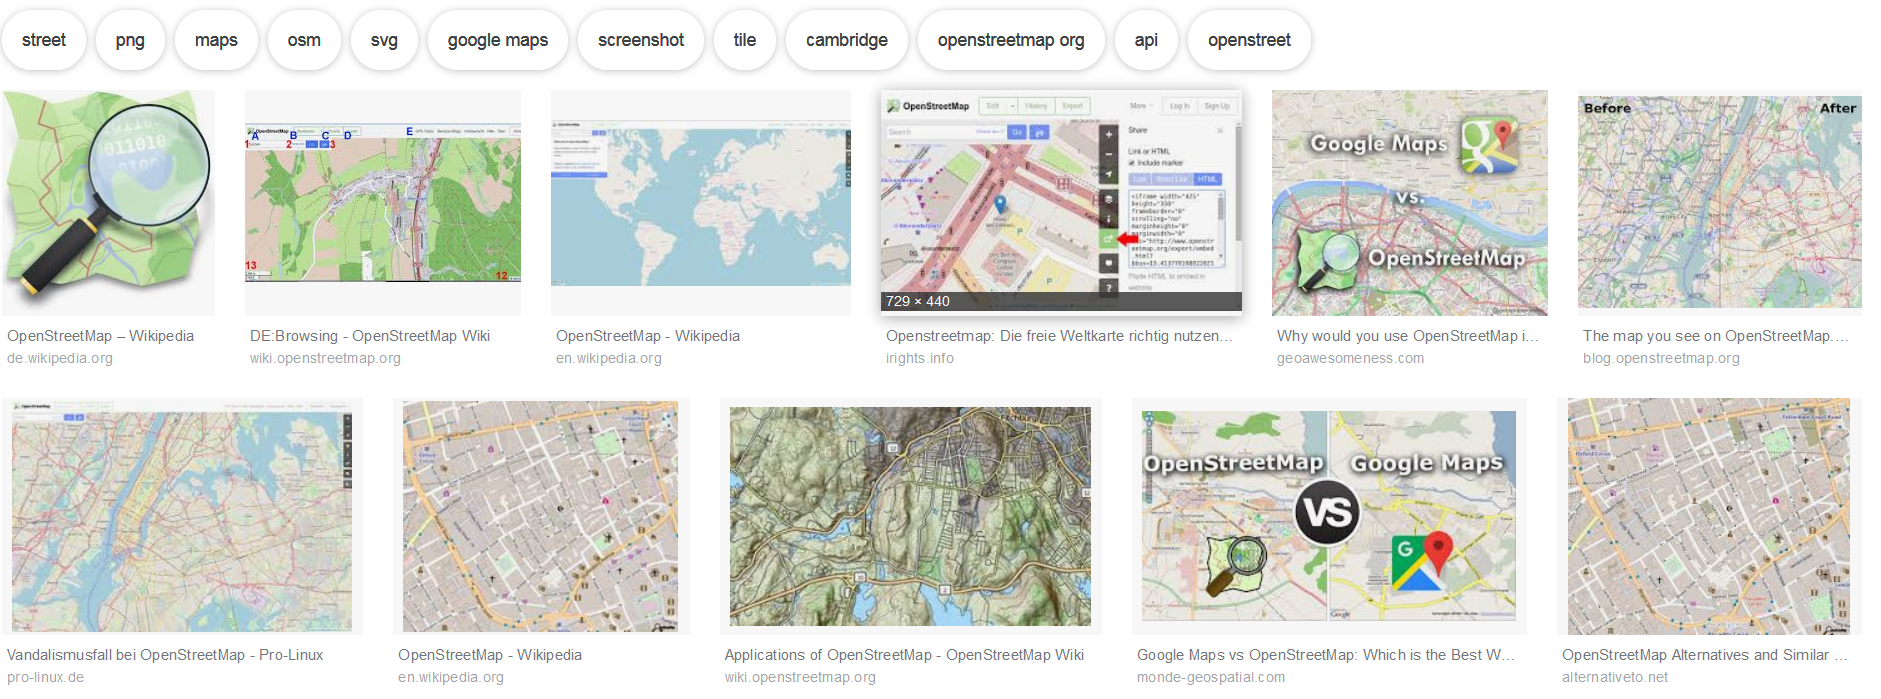
\includegraphics{figure/overview_osm.PNG}

\end{block}

\end{frame}

\begin{frame}{\href{https://wiki.openstreetmap.org/wiki/Tags}{Openstreetmap
Tags}}
\protect\hypertarget{openstreetmap-tags}{}

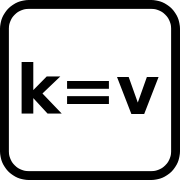
\includegraphics{figure/osm_tag.png}

\end{frame}

\begin{frame}{\href{http://wiki.openstreetmap.org/wiki/DE:Map_Features}{OSM
Map Features}}
\protect\hypertarget{osm-map-features}{}

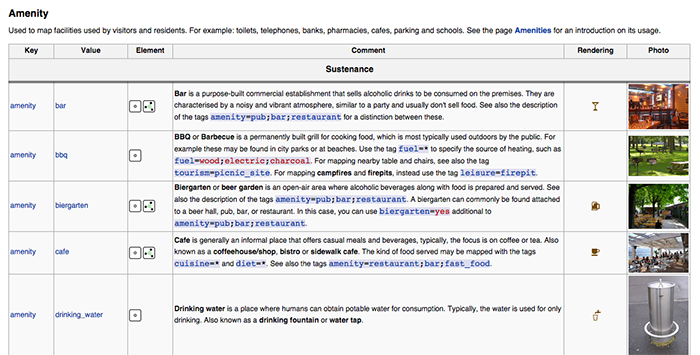
\includegraphics{figure/osm_mapfeatures.png}

\end{frame}

\begin{frame}{Objekttypen in OSM}
\protect\hypertarget{objekttypen-in-osm}{}

\begin{block}{Es gibt prinipiell drei verschiedene Objekttypen:}

\begin{itemize}
\tightlist
\item
  nodes (points),
\item
  ways (polygons and polylines)
\item
  relations (logical grouping of all three object types to express
  real-world geographical relationships)
\end{itemize}

Hippolyte Pruvost and Peter Mooney: Exploring Data Model Relations in
OpenStreetMap

\end{block}

\end{frame}

\begin{frame}{OpenStreetMap objects}
\protect\hypertarget{openstreetmap-objects}{}

\begin{block}{\href{https://www.slideshare.net/mvexel/openstreetmap-9819440}{\textbf{Martijn
van Exel}}}

\begin{itemize}
\tightlist
\item
  nodes and ways
\end{itemize}

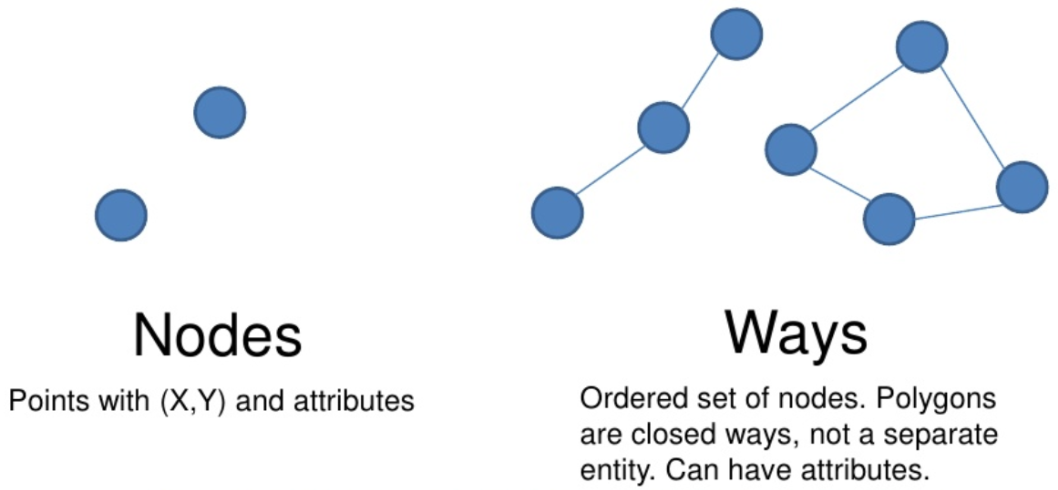
\includegraphics{figure/Nodes_ways.PNG}

\end{block}

\end{frame}

\begin{frame}{OpenStreetMap objects}
\protect\hypertarget{openstreetmap-objects-1}{}

\begin{block}{Relations}

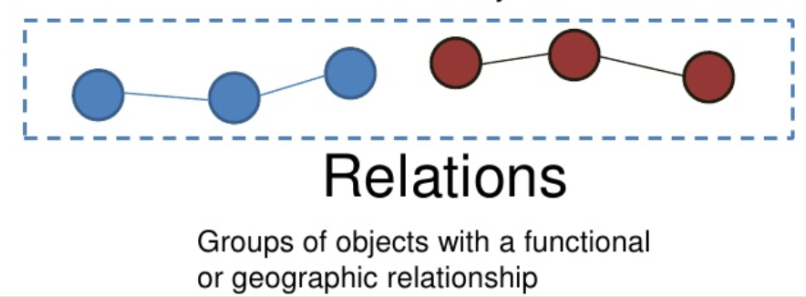
\includegraphics{figure/relations.PNG}

\end{block}

\end{frame}

\begin{frame}{Download von OpenStreetMap Daten -
\href{https://mapzen.com/}{Metro extracts}}
\protect\hypertarget{download-von-openstreetmap-daten---metro-extracts}{}

\begin{itemize}
\tightlist
\item
  Ausschnitte von OpenStreetMap für einzelne Städte
  (\href{https://mapzen.com/data/metro-extracts/}{\textbf{metro
  extracts}})
\end{itemize}

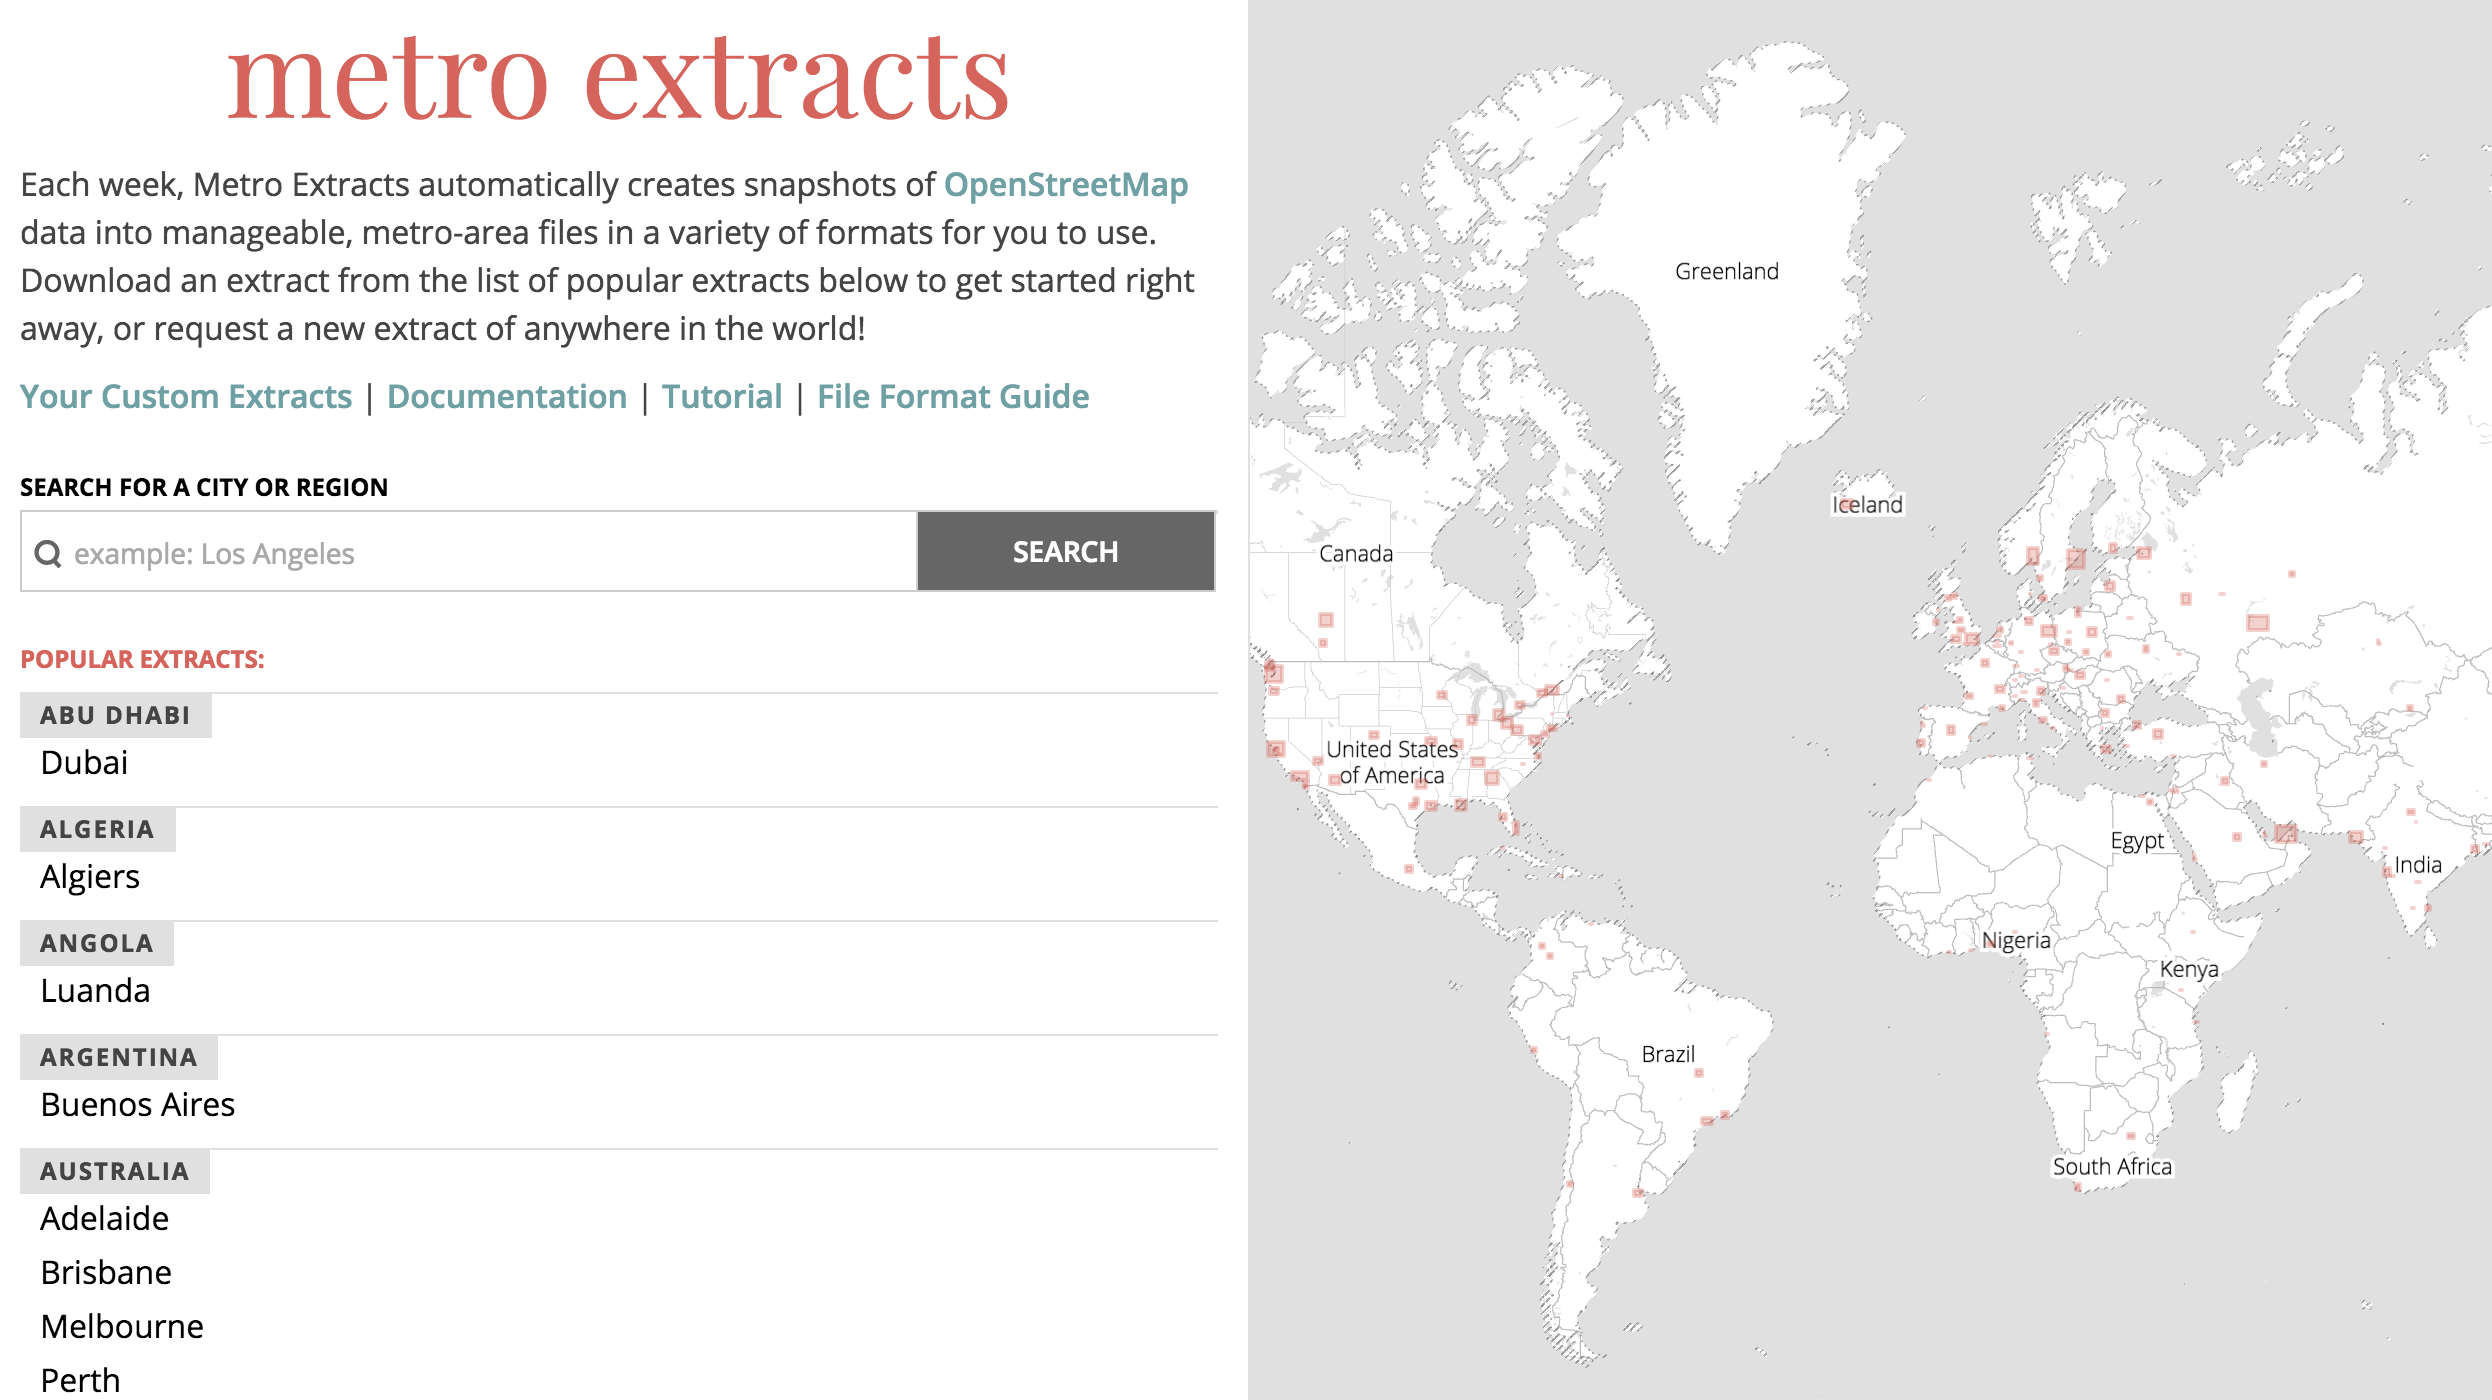
\includegraphics{figure/metroextracts.png}

\end{frame}

\begin{frame}{Download von OpenStreetMap Daten - Geofabrik}
\protect\hypertarget{download-von-openstreetmap-daten---geofabrik}{}

\begin{block}{Geofabrik}

\begin{itemize}
\tightlist
\item
  Über \href{http://download.geofabrik.de/}{\textbf{Geofabrik}} lassen
  sich aktuelle Ausschnitte (auch Shapefiles) herunterladen
\end{itemize}

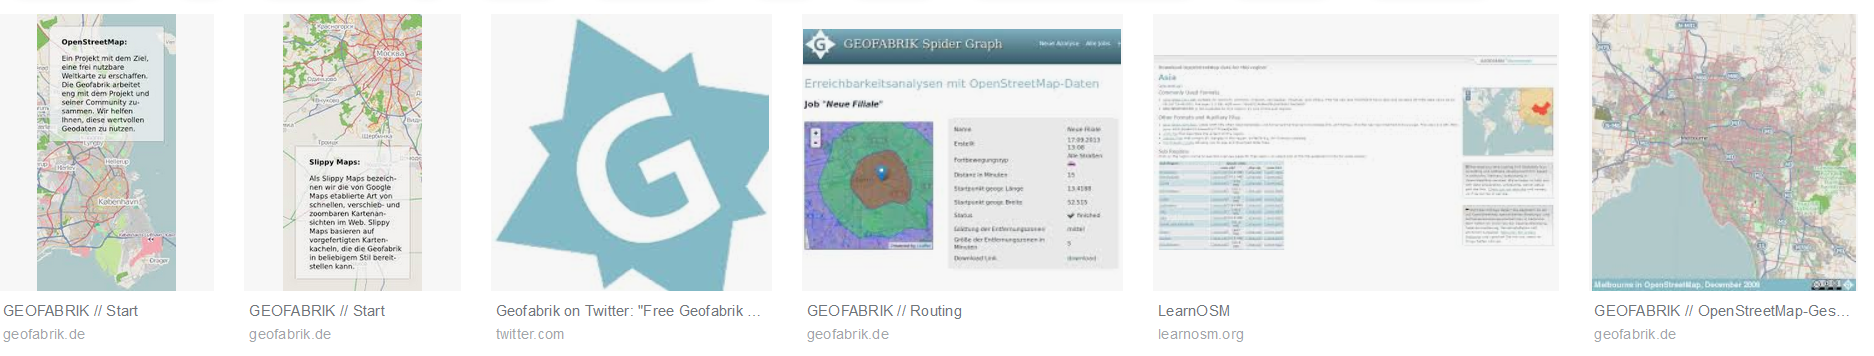
\includegraphics{figure/Geofabrik.PNG}

\end{block}

\end{frame}

\begin{frame}{Download von OpenStreetMap Daten - openaprs}
\protect\hypertarget{download-von-openstreetmap-daten---openaprs}{}

\begin{block}{Kartendaten
(\href{http://www.openaprs.net/}{\textbf{openaprs}})}

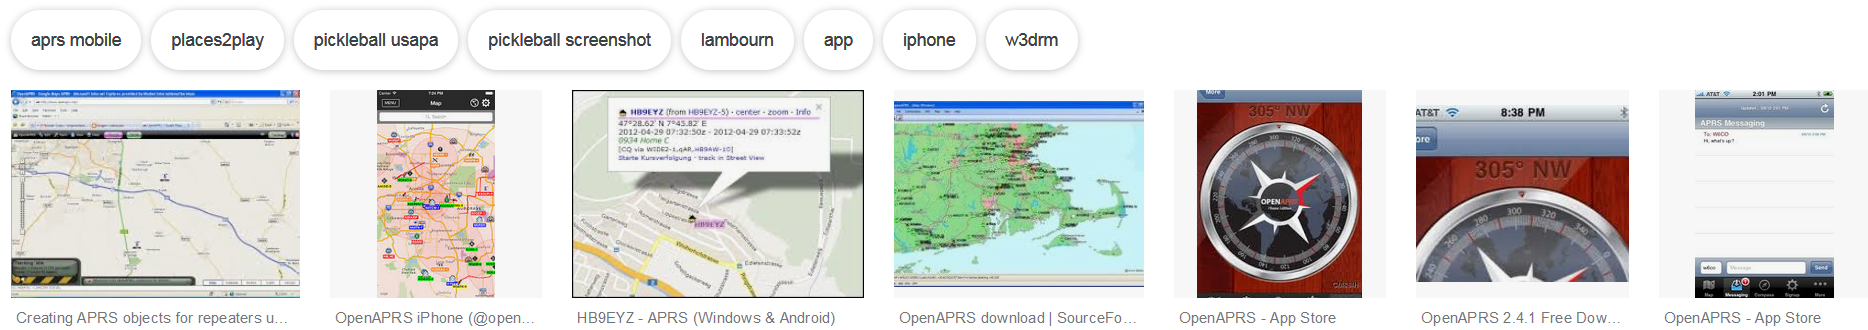
\includegraphics{figure/openaprs.PNG}

\end{block}

\end{frame}

\begin{frame}{OSM Planet file}
\protect\hypertarget{osm-planet-file}{}

\begin{block}{Datenbanklösungen}

\begin{itemize}
\tightlist
\item
  Bei den eben vorgestellten Möglichkeiten geht es vor allem um das
  Herunterladen kleiner Ausschnitte.
\item
  Wenn größere Datenmengen benötigt werden, sollte man eine
  Datenbanklösung nutzen.
\item
  \href{http://www.postgresql.org/}{\textbf{PostgreSQL}} hat den
  Vorteil, dass es Open-Source ist.
\end{itemize}

\end{block}

\end{frame}

\begin{frame}{\href{http://www.postgresql.org/download/windows/}{Download
PostreSQL}}
\protect\hypertarget{download-postresql}{}

\begin{itemize}
\tightlist
\item
  \href{https://datashenanigan.wordpress.com/2015/05/18/getting-started-with-postgresql-in-r/}{\textbf{Hier}}
  ist eine Einführung in PostgreSQL zu finden
\end{itemize}

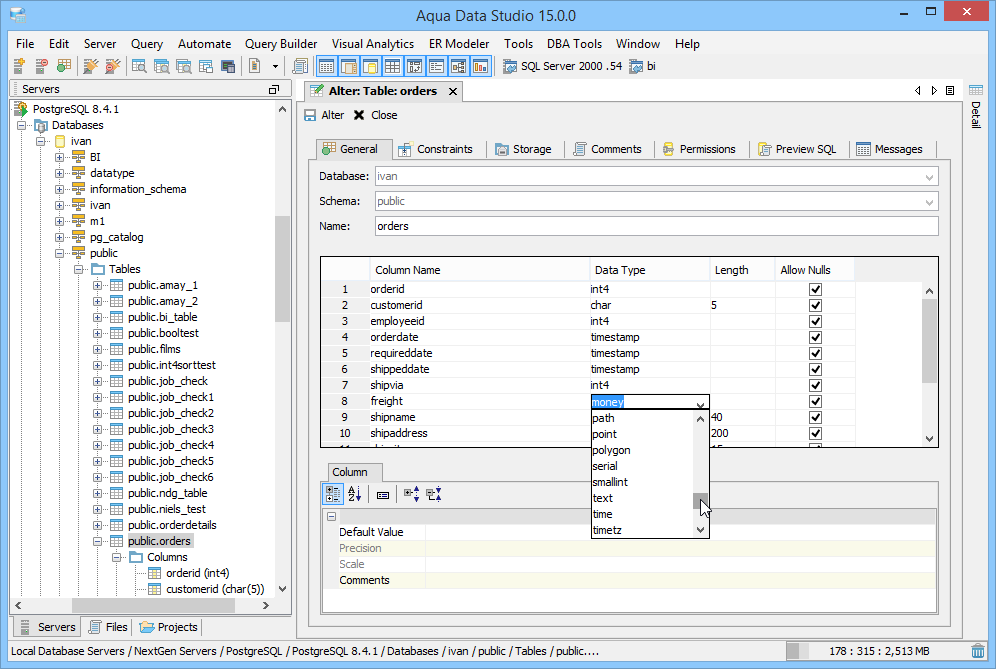
\includegraphics{figure/aquadatastudio_postgresql_visual_table_editing.png}

\end{frame}

\begin{frame}{pgAdmin}
\protect\hypertarget{pgadmin}{}

\begin{itemize}
\tightlist
\item
  Sehr empfehlenswert: Arbeiten mit
  \href{https://www.pgadmin.org/}{\textbf{pgAdmin}}
\item
  Beispiel: um Verknüpfung zu einer Datenbank herzustellen - Doppelklick
  auf den Server in pgAdmin
\end{itemize}

\end{frame}

\begin{frame}[fragile]{PostGIS für PostgreSQL}
\protect\hypertarget{postgis-fur-postgresql}{}

\begin{itemize}
\tightlist
\item
  \href{http://postgis.net/install/}{\textbf{Installieren}} der PostGIS
  Erweiterung:
\end{itemize}

\begin{verbatim}
CREATE EXTENSION postgis;
\end{verbatim}


\includegraphics{figure/PostGIS_logo.png}

\end{frame}

\begin{frame}[fragile]{Programm zum Import der OSM Daten in PostgreSQL-
osm2pgsql}
\protect\hypertarget{programm-zum-import-der-osm-daten-in-postgresql--osm2pgsql}{}

\begin{itemize}
\tightlist
\item
  Läuft unter Linux deutlich besser
\item
  so könnte bspw. ein Import in PostgreSQL aussehen:
\end{itemize}

\begin{verbatim}
osm2pgsql -c -d osmBerlin --slim -C  -k  berlin-latest.osm.pbf
\end{verbatim}

\end{frame}

\begin{frame}[fragile]{Verbindung zwischen R und Postrgesql}
\protect\hypertarget{verbindung-zwischen-r-und-postrgesql}{}

\begin{Shaded}
\begin{Highlighting}[]
\KeywordTok{install.packages}\NormalTok{(}\StringTok{"RPostgreSQL"}\NormalTok{)}
\end{Highlighting}
\end{Shaded}

\begin{Shaded}
\begin{Highlighting}[]
\KeywordTok{library}\NormalTok{(}\StringTok{"RPostgreSQL"}\NormalTok{)}
\end{Highlighting}
\end{Shaded}

\begin{itemize}
\item
  \href{https://github.com/tomoakin/RPostgreSQL}{\textbf{Github
  Verzeichnis}} zum Paket \#\# Nutze bspw.
  \href{http://www.qgis.org/de/site/}{QGIS} um Shapefiles zu extrahieren
\item
  \href{http://www.qgistutorials.com/de/docs/downloading_osm_data.html}{Plugin
  OpenLayers}
\end{itemize}

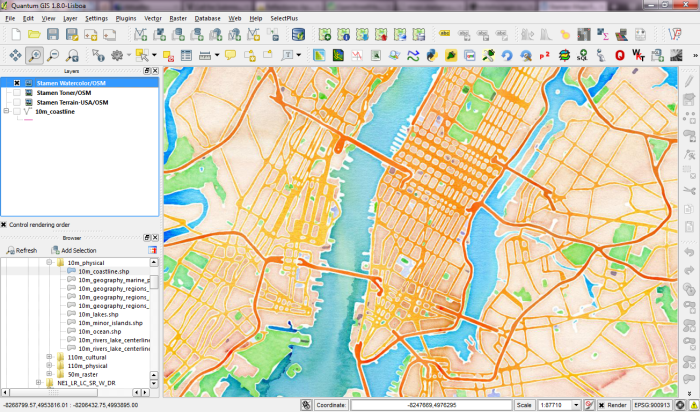
\includegraphics{figure/stamen_watercolor1.png}

\end{frame}

\begin{frame}{Links}
\protect\hypertarget{links}{}

\begin{itemize}
\item
  \href{http://wiki.openstreetmap.org/wiki/Downloading_data}{\textbf{Wiki
  zum Downlaod}} von Openstreetmap Daten
\item
  \href{http://blog.openstreetmap.de/}{\textbf{Openstreetmap Blog}}
\item
  Liste möglicher Datenquellen für räumliche Analysen
  (\href{http://wiki.openstreetmap.org/wiki/Potential_Datasources}{weltweit}
  und in
  \href{http://wiki.openstreetmap.org/wiki/DE:Potential_Datasources}{\textbf{Deutschland}}
  )
\item
  \href{http://wiki.openstreetmap.org/wiki/SALB}{\textbf{SALB}} -
  Administrative Grenzen
\end{itemize}

\url{http://wiki.openstreetmap.org/wiki/SALB}

\end{frame}

\end{document}
